% la-05-leastsqu.tex

\documentclass[xcolor=dvipsnames]{beamer}
\usepackage{teachbeamer}

\title{Least Squares Method}
\subtitle{{\CourseNumber}, BCIT}

\author{\CourseName}

\date{October 12, 2018}

\begin{document}

\begin{frame}
  \titlepage
\end{frame}

\begin{frame}
  \frametitle{Projection}
  The \alert{projection} $u_{H}$ of a vector $u$ onto a hyperplane $H$
  is the vector in the hyperplane that is ``most similar'' to $u$. The
  formal definition for $u_{H}$ requires that
  \begin{enumerate}
  \item $u$ is in $H$
  \item $(u-u_{H})$ is orthogonal to all basis vectors of $H$
  \end{enumerate}
\end{frame}

\begin{frame}
  \frametitle{Projection}
  \beispiel{Finding a Projection} Let $H$ be the line spanned by
  $\vec{v}=(-1,1)^{\intercal}$ in $\mathbb{R}^{2}$. What is the
  projection $\vec{w}$ of $\vec{u}=(3,-2)^{\intercal}$?
    \begin{figure}[h]
    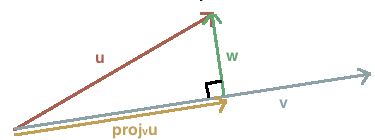
\includegraphics[scale=0.32]{./diagrams/project.png}
  \end{figure}
  Let $\vec{w}=(w_{1},w_{2})^{\intercal}$. Then (1) $\vec{u}-\vec{w}$
  is orthogonal to $\vec{v}$ and (2) $\vec{w}=\alpha\vec{v}$ for some
  $\alpha\in\mathbb{R}$.
  \begin{equation}
    \label{eq:vorahcat}
    \begin{array}{ccccc}
      w_{1}&-&w_{2}&=&5 \\
      w_{1}&+&w_{2}&=&0 \\
    \end{array}
  \end{equation}
Cramer's rule tells us that $\vec{w}=(2.5,-2.5)^{\intercal}$. 
\end{frame}

\begin{frame}
  \frametitle{Projection}
  Let $u=(u_{1},{\ldots},u_{n})^{\intercal}$ be a vector and $H$ be a
  $k$-dimensional hyperplane in the vector space $\mathbb{R}^{n}$. Let
  $x_{1},{\ldots},x_{k}$ be a basis for $H$. Then it is true for all
  vectors $v$ in the hyperplane that
  \begin{equation}
    \label{eq:ahdoogoh}
    \Vert{}u-v\Vert\geq\Vert{}u-u_{H}\Vert
  \end{equation}
  Proof: use the theorem of Pythagoras for
  \begin{equation}
    \label{eq:yoochaev}
    \Vert{}u-v\Vert^{2}=\Vert{}u-u_{H}\Vert^{2}+\Vert{}u_{H}-v\Vert^{2}\geq\Vert{}u-u_{H}\Vert^{2}
  \end{equation}
The claim follows. It illustrates what I mean when I say that $u_{H}$
is the vector in $H$ that is most similar to $u$. 
\end{frame}

\begin{frame}
  \frametitle{Projection}
  \beispiel{Finding Another Projection} What is the projection of
  $\vec{u}=(5,2,10)^{\intercal}$ onto the plane $T$ characterized by
  $2x+y+3z=0$?

  \medskip

  First we find two linearly independent vectors in $H$ to form a
  basis of $H$, for example $\vec{v_{1}}=(1,1,-1)^{\intercal}$ and
  $\vec{v_{2}}=(0,-3,1)^{\intercal}$. The conditions
  \begin{enumerate}
  \item $u_{H}\in{}T$
  \item $(u-u_{H})\perp{}v_{1}$
  \item $(u-u_{H})\perp{}v_{2}$
  \end{enumerate}
  give us the system of linear equations
  \begin{equation}
    \label{eq:faishiso}
    \left[
      \begin{array}{ccc}
        2 & 1 & 3 \\
        -1 & 1 & 1 \\
        0 & 3 & -1
      \end{array}\right]\cdot\left[
      \begin{array}{c}
        \hat{x} \\
        \hat{y} \\
        \hat{z}
      \end{array}\right]=\left[
      \begin{array}{c}
        0 \\
        3 \\
        -4
      \end{array}\right]
  \end{equation}
for which the solution is $u_{H}=(\hat{x},\hat{y},\hat{z})^{\intercal}=(-1,-1,1)^{\intercal}$.
\end{frame}

\begin{frame}
  \frametitle{Projection}
  Let there be two linearly independent vectors $u$ and $v$ in
  $\mathbb{R}^{n}$. Then the formula for the projection $u_{v}$ of $u$ onto
  the line spanned by $v$ is
  \begin{equation}
    \label{eq:weehohqu}
    u_{v}=\left(\frac{u\cdot{}v}{v\cdot{}v}\right)v
  \end{equation}
To verify the formula, note that $u_{v}=av$ for some real number $a$.
Therefore
\begin{equation}
  \label{eq:yahveego}
  (u-av)\perp{}v
\end{equation}
Isolate $a$ in the equation $(u-av)\cdot{}v=0$ to yield the formula.
\end{frame}

\begin{frame}
  \frametitle{Projection}
  Formula (\ref{eq:weehohqu}) only works when the hyperplane is a
  line. You can scale up the idea in terms of dimensions by the
  following theorem.
  \begin{block}{Formula for Projection Onto Plane with Orthogonal
      Basis}
    Let $\{u,v\}$ be an orthogonal basis for $H$. Then the projection
    of $w$ onto $H$ is the sum of $w_{u}$ and $w_{v}$, the projections
    of $w$ onto the lines spanned by $u$ and $v$, respectively.
  \end{block}
  Proof: check the following
  \begin{enumerate}
  \item $(w_{u}+w_{v})\in{}H$ (trivial)
  \item $(w-(w_{u}+w_{v}))\perp{}u$ (use the fact that $u\perp{}v$)
  \item $(w-(w_{u}+w_{v}))\perp{}v$ (same idea)
  \end{enumerate}
\end{frame}

\begin{frame}
  \frametitle{Least Squares Method}
  Consider the following table of measurements for the length of shoe
  prints and the height of the person wearing the shoes.

  \medskip
  
  \begin{tabular}{|c|c|}\hline
    Shoe Print (cm) & Height (cm) \\ \hline
    29.7 & 175.3 \\ \hline
    29.9 & 177.8 \\ \hline
    31.4 & 185.4 \\ \hline
    31.8 & 175.3 \\ \hline
    27.6 & 172.7 \\ \hline
  \end{tabular}

  \medskip
  
  In the statistics portion of this course, we will learn whether the
  paired data provide evidence of a linear relationship. In the linear
  algebra portion, we will learn how to find the line which is closest
  to the data points in the least squares sense.
\end{frame}

\begin{frame}
  \frametitle{Least Squares Method}
    \begin{figure}[h]
    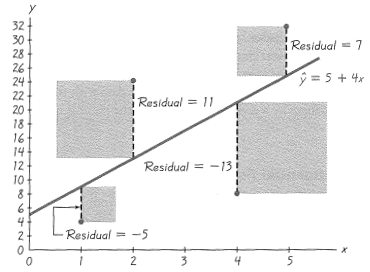
\includegraphics[scale=1]{./diagrams/lsqu4.png}
    \end{figure}
\end{frame}

% \begin{frame}
%   \frametitle{Least Squares Method}
%     \begin{figure}[h]
%     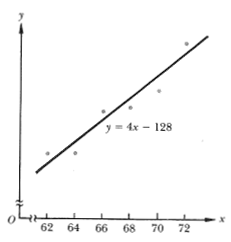
\includegraphics[scale=1]{./diagrams/lsqu1.png}
%     \end{figure}
% \end{frame}

% \begin{frame}
%   \frametitle{Least Squares Method}
%     \begin{figure}[h]
%     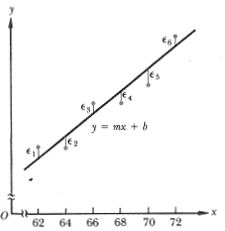
\includegraphics[scale=1]{./diagrams/lsqu3.png}
%     \end{figure}
% \end{frame}

\begin{frame}
  \frametitle{Least Squares Method}
  \begin{block}{Least Squares Method}
    If $L$ is a given line, the \alert{error} for each data point is
    the vertical distance from that point to the line. The
    \alert{squared error} is the sum of the squares of the errors. The
    line that best fits the data in the least squares sense is the
    line that minimizes the squared error.
  \end{block}

  \bigskip

  You can find the \alert{regression line} using calculus
  optimization. However, there is also an elegant method using linear
  algebra.
\end{frame}

\begin{frame}
  \frametitle{Least Squares Method}
  Let $L$ be a line with slope $m$ and $y$-intercept $b$. Let
  $(x_{1},y_{1}),(x_{2},y_{2}),{\ldots},(x_{n},y_{n})$ be a set of
  paired data. Then the following equations hold:
  \begin{equation}
    \label{eq:cheexame}
    \begin{array}{ccccccc}
      y_{1}&=&mx_{1}&+&b&+&\epsilon_{1} \\
      y_{2}&=&mx_{2}&+&b&+&\epsilon_{2} \\
      &&&{\vdots}&&& \\
      y_{n}&=&mx_{n}&+&b&+&\epsilon_{n} \\
    \end{array}
  \end{equation}
where the $\epsilon_{i}$ are the errors ($i=1,{\ldots},n$). This
system is equivalent to the following vector equation,
\begin{equation}
  \label{eq:aewieley}
  Y=AV+E
\end{equation}
where $Y,A,V,E$ are defined on the next slide.
\end{frame}

\begin{frame}
  \frametitle{Least Squares Method}
  \begin{equation}
    \label{eq:aikaewah}
    Y=\left[
      \begin{array}{cc}
        y_{1}  \\
        y_{2}  \\
        {\vdots} \\
        y_{n}  
      \end{array}\right],
    A=\left[
      \begin{array}{cc}
        x_{1} & 1 \\
        x_{2} & 1 \\
        {\vdots} & {\vdots} \\
        x_{n} & 1
      \end{array}\right],
    V=\left[
      \begin{array}{cc}
        m  \\
        b  
      \end{array}\right],
    E=\left[
      \begin{array}{cc}
        \epsilon_{1}  \\
        \epsilon_{2}  \\
        {\vdots} \\
        \epsilon_{n}  
      \end{array}\right]\notag
  \end{equation}
  $E$ is called the error vector. According to (\ref{eq:aewieley}), it
  is
  \begin{equation}
    \label{eq:keebiero}
    E=Y-AV
  \end{equation}
  We are trying to choose $m,b$ so that
  \begin{equation}
    \label{eq:phugeyai}
    \Vert{}E\Vert^{2}=\Vert{}Y-AV\Vert^{2}
  \end{equation}
is minimal.
\end{frame}

\begin{frame}
  \frametitle{Least Squares Method}
  Let
  \begin{equation}
    \label{eq:iapuveer}
    X=\left[
      \begin{array}{c}
        x_{1} \\
        {\vdots} \\
        x_{n}
      \end{array}\right]\mbox{ and }B=\left[
      \begin{array}{c}
        1 \\
        {\vdots} \\
        1
      \end{array}\right]
  \end{equation}
  Then $AV=mX+bB$. The set $S=\{AV|m,b\in\mathbb{R}\}$ is a plane in
  $n$-dimensional space. The ordered pair $(m,b)$ that minimizes the
  squared error corresponds to the projection $Y_{S}$ of $Y$ onto $S$.
\end{frame}

\begin{frame}
  \frametitle{Least Squares Method}
  Let $C$ be $B-B_{X}$, where $B_{X}$ is the projection of $B$ onto
  the line spanned by $X$. Then
  \begin{equation}
    \label{eq:aiwaozie}
    C=B-\left(\frac{B\cdot{}X}{X\cdot{}X}\right)X
  \end{equation}
  Note that $X\perp{}C$. $X$ and $C$ form an orthogonal basis for $S$.
  We have chosen $C$ by a process called \alert{successive orthogonal
    selection}. Consequently,
  \begin{equation}
    \label{eq:eijohkah}
    Y_{S}=Y_{X}+Y_{C}=\left(\frac{Y\cdot{}X}{X\cdot{}X}\right)X+\left(\frac{Y\cdot{}C}{C\cdot{}C}\right)C
  \end{equation}
\end{frame}

\begin{frame}
  \frametitle{Least Squares Method}
  Replace the rightmost $C$ by $B-\left(\frac{B\cdot{}X}{X\cdot{}X}\right)X$ for
  \begin{equation}
    \label{eq:maigeise}
    Y_{S}=\left(\frac{Y\cdot{}X}{X\cdot{}X}-\left(\frac{Y\cdot{}C}{C\cdot{}C}\right)\left(\frac{B\cdot{}X}{X\cdot{}X}\right)\right)X+\left(\frac{Y\cdot{}C}{C\cdot{}C}\right)B
  \end{equation}
  or alternatively
  \begin{equation}
    \label{eq:soguesee}
    m=\frac{Y\cdot{}X}{X\cdot{}X}-\left(\frac{Y\cdot{}C}{C\cdot{}C}\right)\left(\frac{B\cdot{}X}{X\cdot{}X}\right)
  \end{equation}
  \begin{equation}
    \label{eq:cuboonai}
    b=\frac{Y\cdot{}C}{C\cdot{}C}
  \end{equation}
  with
  \begin{equation}
    \label{eq:nesheeli}
    C=B-\left(\frac{B\cdot{}X}{X\cdot{}X}\right)X
  \end{equation}
\end{frame}

\begin{frame}
  \frametitle{Shoe Print and Height}
  \beispiel{Shoe Print and Height} Recall

    \begin{tabular}{|c|c|}\hline
    Shoe Print (cm) & Height (cm) \\ \hline
    29.7 & 175.3 \\ \hline
    29.9 & 177.8 \\ \hline
    31.4 & 185.4 \\ \hline
    31.8 & 175.3 \\ \hline
    27.6 & 172.7 \\ \hline
  \end{tabular}

  Which \alert{regression line} best represents a possible linear
  relationship between shoe print and height? In this case, the shoe
  print is the independent variable $x$, on the basis of which we are
  trying to predict the dependent variable $y$, the height.
  \begin{equation}
    \label{eq:ohngahse}
    X=\left[
      \begin{array}{c}
    29.7 \\
    29.9 \\
    31.4 \\
    31.8 \\
    27.6
      \end{array}\right],Y=\left[
      \begin{array}{c}
    175.3 \\
    177.8 \\
    185.4 \\
    175.3 \\
    172.7 
      \end{array}\right],B=\left[
      \begin{array}{c}
    1 \\
    1 \\
    1 \\
    1 \\
    1 
      \end{array}\right]
  \end{equation}
\end{frame}

\begin{frame}
  \frametitle{Shoe Print and Height}
  Calculate $C$ using the formula
  \begin{equation}
    \label{eq:chawohph}
    C=B-\left(\frac{B\cdot{}X}{X\cdot{}X}\right)X=\left[
      \begin{array}{c}
   0.0150340 \\
   0.0084012 \\
  -0.0413445 \\
  -0.0546101 \\
   0.0846780
      \end{array}\right]
  \end{equation}
  Now calculate $m$ and $b$
    \begin{equation}
    \label{eq:thoemeir}
    m=\frac{Y\cdot{}X}{X\cdot{}X}-\left(\frac{Y\cdot{}C}{C\cdot{}C}\right)\left(\frac{B\cdot{}X}{X\cdot{}X}\right)=1.7528
  \end{equation}
  \begin{equation}
    \label{eq:ohwoiwoh}
    b=\frac{Y\cdot{}C}{C\cdot{}C}=124.58
  \end{equation}
\end{frame}

\begin{frame}
  \frametitle{Shoe Print and Height}
      \begin{figure}[h]
    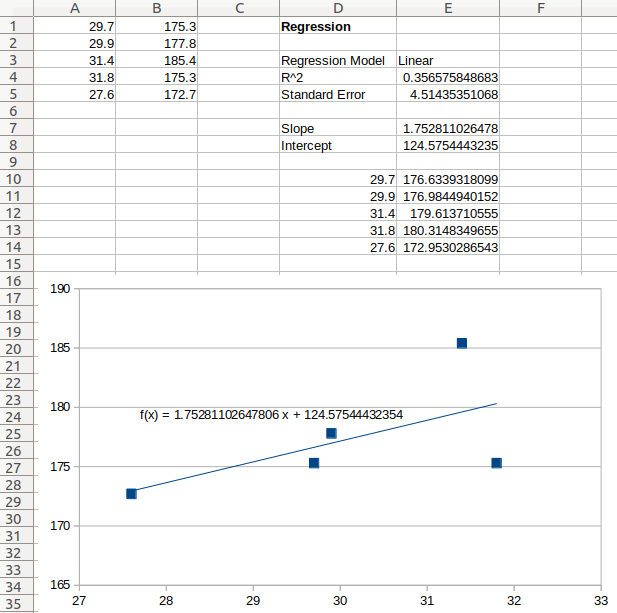
\includegraphics[scale=0.4]{./diagrams/librelinreg.png}
  \end{figure}
\end{frame}

\begin{frame}
  \frametitle{Angles at Gray Cliff}
  \beispiel{Angles at Gray Cliff} This example is from \mbox{Oscar S.
    Adams's} \emph{Application of the Theory of Least Squares to the
    Adjustment of Triangulation} (1915), a ``working manual for the
  computer in the office.'' You measure the following angles.

  \medskip
  
  \begin{tabular}{|c|c|c|}\hline
    from & to & angle \\ \hline
    Boulder & Tower & $65^{\circ}6'29.3''$ \\ \hline
    Tower & Tyonek & $19^{\circ}46'26.9''$ \\ \hline
    Tyonek & Round Point & $8^{\circ}39'14.2''$ \\ \hline
    Round Point & Boulder & $266^{\circ}27'47.9''$ \\ \hline
    % Boulder & Round Point & $93^{\circ}32'9.6''$ \\ \hline
  \end{tabular}
\end{frame}

\begin{frame}
  \frametitle{Angles at Gray Cliff}
  Notice that the angles do not add up to $360^{\circ}$. We are
  missing $1.7''$. How should we adjust these numbers?

  \medskip

  Basic assumptions underlying least squares theory in surveying are
  \begin{enumerate}
  \item mistakes and systematic errors have been eliminated
  \item the number of observations being adjusted is large
  \item the frequency distribution of the errors is normal
  \end{enumerate}
\end{frame}

\begin{frame}
  \frametitle{Angles at Gray Cliff}
  Convert the angles to real numbers
  \begin{equation}
    \label{eq:maeshoga}
    \hat{a}=65.108,\hat{b}=19.774,\hat{c}=8.6539,\hat{d}=266.46
  \end{equation}
  The sum is $359.999527778$. Here is a system of equations with
  measurement errors, exploiting the fact that $d$ is supposed to be
  $360^{\circ}-(a+b+c)$
\begin{equation}
  \label{eq:puzeiboo}
  \begin{array}{ccc}
    a&=&65.108+\epsilon_{1} \\
    b&=&19.774+\epsilon_{2} \\
    c&=&8.6539+\epsilon_{3} \\
    360-(a+b+c)&=&266.46+\epsilon_{4}
  \end{array}
\end{equation}
\end{frame}

\begin{frame}
  \frametitle{Angles at Gray Cliff}
The system of equations is equivalent to the following matrix
equation.
\begin{equation}
  \label{eq:ijuniero}
  \left[
    \begin{array}{ccc}
      1 & 0 & 0 \\
      0 & 1 & 0 \\
      0 & 0 & 1 \\
      -1 & -1 & -1
    \end{array}\right]\left[
    \begin{array}{c}
      a \\
      b \\
      c
    \end{array}\right]=\left[
    \begin{array}{c}
      65.108 \\
      19.774 \\
      8.6539 \\
      -93.537
    \end{array}\right]+\left[
    \begin{array}{c}
      \epsilon_{1} \\
      \epsilon_{2} \\
      \epsilon_{3} \\
      \epsilon_{4}
    \end{array}\right]
\end{equation}
In symbols,
\begin{equation}
  \label{eq:eceesien}
  AV=Y+E
\end{equation}
Again, we want to minimize
\begin{equation}
  \label{eq:ahgaituc}
  \Vert{}Y-AV\Vert^{2}=\Vert{}E\Vert^{2}
\end{equation}
\end{frame}

\begin{frame}
  \frametitle{Angles at Gray Cliff}
  The minimization is achieved by projecting $Y$ onto the hyperplane $S$
  \begin{equation}
    \label{eq:shohyaec}
    a\left[
      \begin{array}{c}
        1 \\
        0 \\
        0 \\
        -1
      \end{array}\right]+b\left[
      \begin{array}{c}
        0 \\
        1 \\
        0 \\
        -1
      \end{array}\right]+c\left[
      \begin{array}{c}
        0 \\
        0 \\
        1 \\
        -1
      \end{array}\right]
  \end{equation}
  These three vectors $\alpha,\beta,\gamma$ form a basis of $S$, but
  the basis vectors are not orthogonal to each other. We will search
  for a different basis of $S$ that is orthonormal by successive
  orthogonal selection.
\end{frame}

\begin{frame}
  \frametitle{Angles at Gray Cliff}
  Start with a non-zero vector $b_{1}$ in $S$, for example
  $b_{1}=\alpha=(1,0,0,-1)^{\intercal}$. This is our first basis
  vector. The second basis vector $b_{2}$ must fulfill
  \begin{enumerate}
  \item $b_{2}\cdot{}b_{1}=0$ (which is equivalent to
    $b_{2}\perp{}b_{1}$)
  \item $b_{2}\in{}S$
  \end{enumerate}
For example, $b_{2}=(1,-1,-1,1)^{\intercal}$ qualifies. Follow the
same procedure for $b_{3}=(0,1,-1,0)^{\intercal}$.
\end{frame}

\begin{frame}
  \frametitle{Angles at Gray Cliff}
  Let $Y_{i}$ be the projection of $Y$ onto the line spanned by
  $b_{i}$, for example. 
  \begin{equation}
    \label{eq:zeoyeobe}
    Y_{1}=\left(\frac{Y\cdot{}b_{1}}{b_{1}\cdot{}b_{1}}\right)b_{1}=\left[
      \begin{array}{c}
        79.32242 \\
        0 \\
        0 \\
        -79.32242
      \end{array}\right]
  \end{equation}
  Then the projection $Y_{S}$ equals $Y_{1}+Y_{2}+Y_{3}=$
  \begin{equation}
    \label{eq:yeeyaesh}
    \left[
      \begin{array}{c}
        79.32242 \\
        0 \\
        0 \\
        -79.32242
      \end{array}\right]+\left[
      \begin{array}{c}
        -14.214 \\
        14.214 \\
        14.214 \\
        -14.214
      \end{array}\right]+\left[
      \begin{array}{c}
        0 \\
        5.56010 \\
        -5.56010 \\
        0
      \end{array}\right]=\left[
      \begin{array}{c}
        65.1083 \\
        19.7743 \\
        8.6541 \\
        -93.5366
      \end{array}\right]\notag
  \end{equation}
  The least squares adjusted angles are
  $65^{\circ}6'29.7'',19^{\circ}46'27.3'',8^{\circ}39'14.6''$ compared
  to the original
  $65^{\circ}6'29.3'',19^{\circ}46'26.9'',8^{\circ}39'14.2''$.
\end{frame}

\begin{frame}
  \frametitle{Abigail, Ben, and Charlie}
  \beispiel{Abigail, Ben, and Charlie} Here is an example adapted from
  \mbox{Paul R. Wolf's} \emph{Survey Measurement Adjustments by Least
    Squares}. Abigail measures a length $\overline{XY}$ to be 211.52 units.
  Ben measures a length $\overline{YZ}$ to be 220.10 units. Charlie
  measures the length $\overline{XZ}$ to be 431.71 units. What lengths
  should they report to their supervisor?

  \medskip

  We will solve this problem three different ways.
  \begin{enumerate}
  \item use calculus
  \item use projection
  \item use a matrix formula based on projection
  \end{enumerate}
\end{frame}

\begin{frame}
  \frametitle{Abigail, Ben, and Charlie [Calculus]}
  Here are the three equations with errors:
  \begin{equation}
    \label{eq:ohjeigoo}
    \begin{array}{ccccc}
      a&&&=&211.52+\epsilon_{1} \\
      &&b&=&220.10+\epsilon_{2} \\
      a&+&b&=&431.71+\epsilon_{3} \\
    \end{array}
  \end{equation}
  Define the function
  \begin{equation}
    \label{eq:ceexaeke}
    F(a,b)=\Vert{}E\Vert^{2}=(a-211.52)^{2}+(b-220.10)^{2}+(a+b-431.71)^{2}=\notag
  \end{equation}
  \begin{equation}
    \label{eq:shaisaht}
    2a^{2}+2ab+2b^{2}-1286.46a-1303.62b+279558.2445
  \end{equation}
  We want to minimize $F$. The partial derivatives are
  \begin{equation}
    \label{eq:ohbiecoa}
    \frac{\partial{}F}{\partial{}a}=4a+2b-1286.46
  \end{equation}
  \begin{equation}
    \label{eq:eureejoo}
    \frac{\partial{}F}{\partial{}b}=2a+4b-1303.62
  \end{equation}
\end{frame}

\begin{frame}
  \frametitle{Abigail, Ben, and Charlie [Calculus]}
  Setting the partial derivatives to zero gives us the following
  system of linear equations.
  \begin{equation}
    \label{eq:megioquo}
    \left[
      \begin{array}{cc}
        4 & 2 \\
        2 & 4
      \end{array}\right]\left[
      \begin{array}{c}
        a \\
        b
      \end{array}\right]=\left[
      \begin{array}{c}
        1286.46 \\
        1303.62
      \end{array}\right]
  \end{equation}
The solution is $a=211.55,b=220.13$ for Abigail and Ben's least
squares adjusted measurements, compared to the original
$\hat{a}=211.52,\hat{b}=220.10$. Charlie's measurement is adjusted
from $431.71$ to $431.68$. 
\end{frame}

\begin{frame}
  \frametitle{Abigail, Ben, and Charlie [Projection]}
  Equation (\ref{eq:ohjeigoo}) translates into the following matrix
  equation.
  \begin{equation}
    \label{eq:eiwiepho}
    \left[
      \begin{array}{cc}
        1 & 0 \\
        0 & 1 \\
        1 & 1 
      \end{array}\right]\left[
      \begin{array}{c}
        a \\
        b
      \end{array}\right]=\left[
      \begin{array}{c}
        211.52 \\
        220.10 \\
        431.71
      \end{array}\right]+\left[
      \begin{array}{c}
        \epsilon_{1} \\
        \epsilon_{2} \\
        \epsilon_{3}
      \end{array}\right]
  \end{equation}
  or
  \begin{equation}
    \label{eq:quahyawi}
    AV=Y+E\mbox{ and therefore }E=Y-AV
  \end{equation}
\end{frame}

\begin{frame}
  \frametitle{Abigail, Ben, and Charlie [Projection]}
  Find the projection $Y_{S}$ of $Y$ onto the hyperplane $S$ defined
  by $AV$ with free variables $a,b$. $u=(1,0,1)^{\intercal}$ and
  $v=(0,1,1)^{\intercal}$ are not orthogonal. Find the projection
  $v_{u}$ of $v$ onto the line spanned by $u$ and define $w=v-v_{u}$
  (successive orthogonal selection).
  \begin{equation}
    \label{eq:ierishie}
    w=v-v_{u}=v-\left(\frac{v\cdot{}u}{u\cdot{}u}\right)u=\left[
      \begin{array}{c}
        -\frac{1}{2} \\
        1 \\
        \frac{1}{2}
      \end{array}\right]
  \end{equation}
  Consequently,
  \begin{equation}
    \label{eq:dieshahz}
    Y_{S}=Y_{u}+Y_{w}=\left(\frac{Y\cdot{}u}{u\cdot{}u}\right)u+\left(\frac{Y\cdot{}w}{w\cdot{}w}\right)w=\left[
      \begin{array}{c}
        211.55 \\
        220.13 \\
        431.68
      \end{array}\right]
  \end{equation}
The solution found by using projection agrees with the solution found by using calculus.
\end{frame}

\begin{frame}
  \frametitle{Abigail, Ben, and Charlie [Linear Algebra]}
  On a rainy day, you may not be in the mood to remember the
  projection procedure. You just want to use a formula. Here it is for
  Abigail, Ben, and Charlie:
  \begin{equation}
    \label{eq:zeifaidu}
    V_{0}=\left[
      \begin{array}{c}
        a \\
        b
      \end{array}\right]=(A^{\intercal}A)^{-1}A^{\intercal}Y=\left[
      \begin{array}{c}
        211.55 \\
        220.13
      \end{array}\right]
  \end{equation}
Why does this formula work?
\end{frame}

\begin{frame}
  \frametitle{Abigail, Ben, and Charlie [Linear Algebra]}
  Let $V_{0}$ be the solution to the least squares problem, $AV_{0}$
  is the projection $Y_{S}$ of $Y$ onto the hyperplane $S$ defined by
  $AV$ when the variables in $V$ are still free. $Y-AV_{0}$ is
  orthogonal to $S$. $S$ is the hyperplane $\{AU|U\mbox{ is a vector
    with the right dimensions}\}$. Consequently,
  \begin{equation}
    \label{eq:aebohche}
    (Y-AV_{0})\cdot{}AU=0
  \end{equation}
  for some $U$ with the right dimensions. Rewrite
  \begin{equation}
    \label{eq:aicohkai}
    Y\cdot{}AU=AV_{0}\cdot{}AU
  \end{equation}
\end{frame}

\begin{frame}
  \frametitle{Abigail, Ben, and Charlie [Linear Algebra]}
For column vectors $u$ and $v$, it is generally true that
$u\cdot{}v=u^{\intercal}\,v$. Also recall that for any two matrices
$A$ and $B$
\begin{equation}
  \label{eq:yaephubo}
    (AB)^{\intercal}=B^{\intercal}A^{\intercal}
\end{equation}
Using these two facts, continue with
\begin{equation}
  \label{eq:ezahsiex}
  Y\cdot{}AU=Y^{\intercal}AU=(A^{\intercal}Y)^{\intercal}U
\end{equation}
and
\begin{equation}
  \label{eq:geexeiri}
  AV_{0}\cdot{}AU=(AV_{0})^{\intercal}AU=(A^{\intercal}AV_{0})^{\intercal}U
\end{equation}
\end{frame}

\begin{frame}
  \frametitle{Abigail, Ben, and Charlie [Linear Algebra]}
Combine (\ref{eq:aicohkai}), (\ref{eq:ezahsiex}) and (\ref{eq:geexeiri}) for
\begin{equation}
  \label{eq:eighaidi}
  (A^{\intercal}Y)^{\intercal}U=(A^{\intercal}AV_{0})^{\intercal}U
\end{equation}
Because this is true for all well-dimensioned vectors $U$, it must be
true that
\begin{equation}
  \label{eq:feizahgh}
  (A^{\intercal}Y)^{\intercal}=(A^{\intercal}AV_{0})^{\intercal}
\end{equation}
If $A^{\intercal}A$ is invertible (this can be shown to be true), it
follows that
\begin{equation}
  \label{eq:waheisha}
  V_{0}=(A^{\intercal}A)^{-1}A^{\intercal}Y
\end{equation}
\end{frame}

\begin{frame}
  \frametitle{Shoe Print and Height}
  Now that we have a formula, let us return to the problem of shoe
  print and height.

  \begin{flushright}
    \begin{tabular}{|c|c|}\hline
    Shoe Print (cm) & Height (cm) \\ \hline
    29.7 & 175.3 \\ \hline
    29.9 & 177.8 \\ \hline
    31.4 & 185.4 \\ \hline
    31.8 & 175.3 \\ \hline
    27.6 & 172.7 \\ \hline
  \end{tabular}
  \end{flushright}

  The yave setup $Y-AV=E$ is
  \begin{equation}
    \label{eq:zeengaip}
    \left[
      \begin{array}{c}
    175.3 \\
    177.8 \\
    185.4 \\
    175.3 \\
    172.7 
      \end{array}\right]-\left[
      \begin{array}{cc}
    29.7 & 1 \\
    29.9 & 1 \\
    31.4 & 1 \\
    31.8 & 1 \\
    27.6 & 1
      \end{array}\right]\left[
      \begin{array}{c}
        m \\
        b
      \end{array}\right]=\left[
    \begin{array}{c}
      \epsilon_{1} \\
      \epsilon_{2} \\
      \epsilon_{3} \\
      \epsilon_{4} \\
      \epsilon_{5}
    \end{array}\right]
  \end{equation}
\end{frame}

\begin{frame}
  \frametitle{Shoe Print and Height}
  Use
  \begin{equation}
    \label{eq:ciephini}
    V_{0}=(A^{\intercal}A)^{-1}A^{\intercal}Y=\left[
      \begin{array}{c}
        1.7528 \\
        124.5754
      \end{array}\right]
  \end{equation}
As we already know, the slope $m$ of the regression line is $1.7528$
and the $y$-intercept $b$ is $124.5754$.
\end{frame}

\begin{frame}
  \frametitle{Least Squares Exercises}
  {\ubung} Find the quadratic of best fit for the data

  \bigskip
  
  \begin{tabular}{c|ccccc}
    x & 0 & 1 & 2 & 3 & 4 \\ \hline
    y & 9.1 & 2.8 & 1.2 & 3.1 & 8.7
  \end{tabular}
  % Paul C. Shields, page 259 solution y=1.95x^2-7.85x+8.98
\end{frame}

\begin{frame}
  \frametitle{Least Squares Exercises}
  {\ubung} At 6327 ft (or 6.327 thousand feet), Mario Triola recorded
  the temperature. Find the best predicted temperature at that
  altitude based on other measurements, assuming a linear
  relationship. How does the result compare to the actual recorded
  value of 48$^{\circ}$F?

% +---------+---------+---------+---------+---------+---------+---------+---------+
% |000      |3        |10       |14       |22       |28       |31       |33       |
% +---------+---------+---------+---------+---------+---------+---------+---------+
% |000      |57       |37       |24       |-5       |-30      |-41      |-54      |
% +---------+---------+---------+---------+---------+---------+---------+---------+

  \bigskip

% This LaTeX table template is generated by emacs 24.5.1
\begin{tabular}{|l|l|l|l|l|l|l|l|}
\hline
Altitude & 3 & 10 & 14 & 22 & 28 & 31 & 33 \\
\hline
Temperature & 57 & 37 & 24 & -5 & -30 & -41 & -54 \\
\hline
\end{tabular}
% Altitude	3	10	14	22	28	31	33
% Temperature	57	37	24	-5	-30	-41	-54
\end{frame}

\begin{frame}
  \frametitle{Least Squares Exercises}
  {\ubung} You measure the four angles in a quadrilateral
  $\hat{a}=8.490426^{\circ},\hat{b}=182.029154^{\circ},\hat{c}=119.148088^{\circ},\hat{d}=50.32948$.
  What are the least squares adjusted measurements?
\end{frame}

\begin{frame}
  \frametitle{Least Squares Exercises}
% Paul R. Wolf, page 501
  {\ubung} Consider the following leveling network. 
    \begin{figure}[h]
    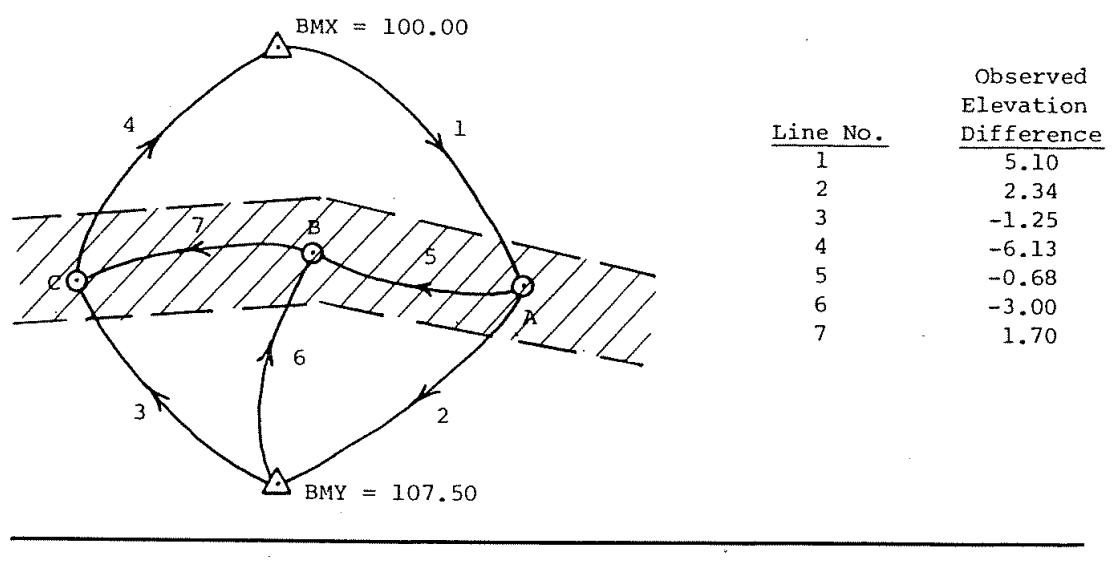
\includegraphics[scale=0.26]{./diagrams/levelingnetwork.png}
  \end{figure}
\end{frame}

\begin{frame}
  \frametitle{Least Squares Exercises}
  The objective is to determine elevations of $A$, $B$, and $C$, which
  are to serve as temporary project bench marks to control
  construction of a highway through the crosshatched corridor.

\bigskip

  Obviously, it would have been possible to obtain elevations for $A$,
  $B$, and $C$ by beginning at $BMX$ and running a single closed loop
  consisting of only courses 1, 5, 7, and 4. Alternatively, a single
  closed loop could have been initiated at $BMY$ and consist of courses
  2, 5, 7, and 3.
\end{frame}

\begin{frame}
  \frametitle{Least Squares Exercises}
  However, by running all seven courses, redundancy is achieved that
  enables checks to be made, blunders to be isolated, and precision to
  be increased. Having run all seven courses, it would be possible to
  compute the adjusted elevation of $B$, for example, using several
  different single closed circuits. Loops 1-5-6, 2-5-6, 3-7-6, and
  4-7-6 could each be used, but it is almost certain that each would
  yield a different elevation for $B$.

\bigskip

  A more logical approach, which will produce only one adjusted value
  for $B$---its most probable one---is to use all seven courses in a
  simultaneous least squares adjustment. In adjusting level networks,
  the observed difference in elevation for each course is treated as
  one observation containing a single random error.
\end{frame}

\begin{frame}
  \frametitle{Least Squares Exercises}
  This single random error is the total of the individual random
  errors in backsight and foresight readings for the entire course. In
  the figure, the arrows indicate the direction of leveling. Thus, for
  course number 1, leveling proceeded from $BMX$ to $A$ and the observed
  elevation difference was $+5.10$ feet.

\bigskip

  Try to find the equations yourself (before looking at the next slide
  to check if they are correct) and then calculate the least squares
  adjusted elevations of $A$, $B$, and $C$.
\end{frame}

\begin{frame}
  \frametitle{Least Squares Exercises}
  The first set of equation for the seven courses is
  \begin{equation}
    \label{eq:aelaeghu}
    \begin{array}{rcl}
      A&=&BMX+5.10+\epsilon_{1} \\
      BMY&=&A+2.34+\epsilon_{2} \\
      C&=&BMY-1.25+\epsilon_{3} \\
      BMX&=&C-6.13+\epsilon_{4} \\
      B&=&A-0.68+\epsilon_{5} \\
      B&=&BMY-3.00+\epsilon_{6} \\
      C&=&B+1.70+\epsilon_{7}
    \end{array}
  \end{equation}
\end{frame}

\begin{frame}
  \frametitle{Least Squares Exercises}
  The resulting yave setup is
  \begin{equation}
    \label{eq:beephaht}
    \begin{array}{rcl}
      A&=&105.10+\epsilon_{1} \\
      A&=&105.16+\epsilon_{2} \\
      C&=&106.25+\epsilon_{3} \\
      C&=&106.13+\epsilon_{4} \\
      A-B&=&0.68+\epsilon_{5} \\
      B&=&104.50+\epsilon_{6} \\
      B-C&=&-1.70+\epsilon_{7}
    \end{array}
  \end{equation}
The adjusted benchmark elevations are $A=105.14,B=104.48,C=106.19$.
\end{frame}

\begin{frame}
  \frametitle{Linearizing Distance Observation Equations}
  \beispiel{Linearizing Equations} You are trying to measure the
  coordinates of stations $A$ and $B$. Your provisional estimate is
  $(8.3995,3.0161)$ and $(-2.872,1.4937)$. Then you observe the length
  between $A$ and $B$ to be $11.391$. How would you report your least
  squares adjusted coordinates for $A$ and $B$, given that you weigh
  equally the errors for $A$ and $B$'s coordinates as well as the
  distance between them?
\end{frame}

\begin{frame}
  \frametitle{Linearizing Distance Observation Equations}
  Setting up the first four yave equations is simple. The fifth one,
  however, is non-linear.
  \begin{equation}
    \label{eq:pheengei}
    \begin{array}{rcl}
      x&=&8.3995+\epsilon_{1} \\
      y&=&3.0161+\epsilon_{2} \\
      z&=&-2.872+\epsilon_{3} \\
      w&=&1.4937+\epsilon_{4} \\
      \sqrt{(z-x)^{2}+(w-y)^{2}}&=&11.391+\epsilon_{5} \\
    \end{array}
  \end{equation}
We shall linearize the fifth equation using the Taylor polynomial
expansion of the function $G(x,y,z,w)=\sqrt{(z-x)^{2}+(w-y)^{2}}$.
\end{frame}

\begin{frame}
  \frametitle{Linearizing Distance Observation Equations}
  Recall the Taylor polynomial expansion of a function
  $f:\mathbb{R}\rightarrow\mathbb{R}$ about $x=a$,
    \begin{equation}
      \label{eq:ahazohve}
      f(x)=f(a)+f'(a)(x-a)+\frac{f''(a)}{2!}(x-a)^{2}+{\ldots}+\notag
    \end{equation}
    \begin{equation}
      \label{eq:oolietai}
      \frac{f^{(n)}(a)}{n!}(x-a)^{n}+{\ldots}
    \end{equation}
To linearize a function $f$, approximate the function only using the
first two terms,
    \begin{equation}
      \label{eq:quaechun}
      f(x)\approx{}f(a)+f'(a)(x-a)
    \end{equation}
\end{frame}

\begin{frame}
  \frametitle{Linearizing Distance Observation Equations}
  Without knowing it, we used Taylor polynomials for Newton's method.
  We were trying to solve $f(x)=0$ but could not because it gave us a
  non-linear equation. Instead, we solved
  \begin{equation}
    \label{eq:vifahtuu}
    f(x)\approx{}f(a)+f'(a)(x-a)=0
  \end{equation}
  which is equivalent to
  \begin{equation}
    \label{eq:noopheij}
    x=a-\frac{f(a)}{f'(a)}
  \end{equation}
This $x$, however, is only an approximation of the true $x$, and so we
repeated the process until we were as close to the $x$-intercept of
$f$ as we needed to be.
\end{frame}

\begin{frame}
  \frametitle{Linearizing Distance Observation Equations}
  The function, however, is a function from
  $\mathbb{R}^{4}\rightarrow\mathbb{R}$.
  \begin{equation}
    \label{eq:oochohda}
G(x,y,z,w)=\sqrt{(z-x)^{2}+(w-y)^{2}}    
  \end{equation}
  We need to use a generalization of Taylor polynomials for higher
  dimensions. Let $F:\mathbb{R}^{n}\rightarrow\mathbb{R}^{m}$. Then
\begin{equation}
  \label{eq:ohvoidei}
 F(\vec{x})=F(\vec{a})+J(\vec{a})(\vec{x}-\vec{a}) 
\end{equation}
where $J$ is the Jacobian matrix
\begin{equation}
  \label{eq:ooveitho}
  J=\left[\begin{array}{ccc}
     \frac{\partial F_1}{\partial x_1} & {\ldots} & \frac{\partial F_1}{\partial x_n} \\
     {\vdots} & {\ddots} & {\vdots} \\
     \frac{\partial F_m}{\partial x_1} & {\ldots} & \frac{\partial F_m}{\partial x_n}
\end{array}\right]
\end{equation}
Note that $F_{i}(\vec{x})=y_{i}$ for $F(\vec{x})=\vec{y}$. 
\end{frame}

\begin{frame}
  \frametitle{Linearizing Distance Observation Equations}
  The Jacobian for $G$ is
  \begin{equation}
    \label{eq:ahchaiyi}
    J(x,y,z,w)=\left[
      \begin{array}{c}
     \frac{x-z}{\sqrt{(z-x)^{2}+(w-y)^{2}}} \\
     \frac{z-x}{\sqrt{(z-x)^{2}+(w-y)^{2}}} \\
     \frac{y-w}{\sqrt{(z-x)^{2}+(w-y)^{2}}} \\
     \frac{w-y}{\sqrt{(z-x)^{2}+(w-y)^{2}}}
      \end{array}\right]^{\intercal}\notag
  \end{equation}
  Therefore
  \begin{equation}
    \label{eq:ziexowei}
    G(x,y,z,w)\approx{}G(\hat{x},\hat{y},\hat{z},\hat{w})+\left[
      \begin{array}{c}
     \frac{\hat{x}-\hat{z}}{\sqrt{(\hat{z}-\hat{x})^{2}+(\hat{w}-\hat{y})^{2}}} \\
     \frac{\hat{y}-\hat{w}}{\sqrt{(\hat{z}-\hat{x})^{2}+(\hat{w}-\hat{y})^{2}}} \\
     \frac{\hat{z}-\hat{x}}{\sqrt{(\hat{z}-\hat{x})^{2}+(\hat{w}-\hat{y})^{2}}} \\
     \frac{\hat{w}-\hat{y}}{\sqrt{(\hat{z}-\hat{x})^{2}+(\hat{w}-\hat{y})^{2}}}
      \end{array}\right]^{\intercal}\left[
      \begin{array}{c}
        x-\hat{x} \\
        y-\hat{y} \\
        z-\hat{z} \\
        w-\hat{w}
      \end{array}\right]\notag
  \end{equation}
\end{frame}

\begin{frame}
  \frametitle{Linearizing Distance Observation Equations}
  It makes sense to use $\hat{x},\hat{y},\hat{z},\hat{w}$ as our first
  estimate for $x,y,z,w$. Therefore, the equation
  \begin{equation}
    \label{eq:jahxiebo}
      \sqrt{(z-x)^{2}+(w-y)^{2}}=11.391+\epsilon_{5}\notag
  \end{equation}
  linearizes to (approximately)
  \begin{equation}
    \label{eq:dooxahru}
    \sqrt{(-2.8724-8.3995)^{2}+(1.4937-3.0161)^{2}}+\notag
  \end{equation}
  \begin{equation}
    \label{eq:eejaetab}
    0.99100(x-8.3995)+0.13385(y-3.0161)-\notag
  \end{equation}
  \begin{equation}
    \label{eq:yahziech}
    0.99100(z+2.8724)-0.13385(w-1.4937)=11.391+\epsilon_{5}\notag
  \end{equation}
  or, equivalently,
  \begin{equation}
    \label{eq:axeeteja}
    0.99100x+0.13385y-0.99100z-0.13385w+0.000018071\notag
  \end{equation}
\end{frame}

\begin{frame}
  \frametitle{Linearizing Distance Observation Equations}
  Finally, we have a linear yave setup.
  \begin{equation}
    \label{eq:hohchadu}
    \left[
      \begin{array}{cccc}
        1&0&0&0 \\
        0&1&0&0 \\
        0&0&1&0 \\
        0&0&0&1 \\
        0.99100&0.13385&-0.99100&-0.13385
      \end{array}\right]\left[
      \begin{array}{c}
        x \\
        y \\
        z \\
        w
      \end{array}\right]=\notag
  \end{equation}
  \begin{equation}
    \label{eq:yaericee}
    \left[
      \begin{array}{c}
8.3995 \\
3.0161 \\
-2.872 \\
        1.4937 \\
        11.391
      \end{array}\right]+\left[
      \begin{array}{c}
      \epsilon_{1} \\
      \epsilon_{2} \\
      \epsilon_{3} \\
      \epsilon_{4} \\
      \epsilon_{5}
    \end{array}\right]
  \end{equation}
\end{frame}

\begin{frame}
  \frametitle{Linearizing Distance Observation Equations}
  Use the formula
  \begin{equation}
    \label{eq:haeyahgo}
    V_{0}=(A^{\intercal}A)^{-1}A^{\intercal}Y
  \end{equation}
  for
  \begin{equation}
    \label{eq:quoiseih}
    V_{0}=(8.4052,3.0169,-2.8777,1.4929)^{\intercal}
  \end{equation}
The least squares adjusted coordinates are
$(8.4052,3.0169)$ and $(-2.8777,1.4929)$, compared to the original
$(8.3995,3.0161)$ and $(-2.8720,1.4937)$.
\end{frame}

\begin{frame}
  \frametitle{Linearizing Angle Observation Equations}
  Next: do this for angles (partial derivative of arctan). Then solve
  system of non-linear equations. Tie this in with Shields, example 2
  on page 296.
\end{frame}

\begin{frame}
  \frametitle{Linearizing Angle Observation Equations}
  \beispiel{Angle Observations} There are three points whose
  coordinates with measurement errors are
  \begin{equation}
    \label{eq:aukoogha}
    \begin{array}{rcl}
      I&=&(595.74,537.76) \\
       J&=&(800.92,658.44) \\
       K&=&(302.96,168.88)
    \end{array}
  \end{equation}
From station $I$, you observe an angle of $158^{\circ}49'21''$ instead
of the expected $158^{\circ}54'5.9107''$ between $\vec{IJ}$ and
$\vec{IK}$. How should you least squares adjust the coordinates of
$I,J,K$ in light of your angle measurement?
\end{frame}

\begin{frame}
  \frametitle{Linearizing Angle Observation Equations}
Compare the original measurements to the least squares adjusted
values.

\bigskip

\begin{tabular}{|r|l|l|}\hline
      $x$&$596.33$&$595.74$ \\ \hline
      $y$&$538.53$&$537.76$ \\ \hline
      $z$&$801.25$&$800.92$ \\ \hline
      $w$&$659.00$&$658.44$ \\ \hline
      $u$&$303.22$&$302.96$ \\ \hline
      $v$&$169.09$&$168.88$ \hline
\end{tabular}
\end{frame}

\begin{frame}
  \frametitle{End of Lesson}
Next Lesson: Eigenvalues and Eigenvectors
\end{frame}

\end{document}
